\documentclass{beamer}

\usetheme{Copenhagen}
\usecolortheme{lily}
\usepackage[T1]{fontenc}
\usepackage[ansinew]{inputenc}
\usepackage[USenglish]{babel}
\usepackage{amsmath}
\usepackage{mathtools}
\usepackage{stmaryrd}
\usepackage{graphicx}
\usepackage{lmodern}

\usepackage[round, authoryear]{natbib}

\newcommand\Wider[2][3em]{%
\makebox[\linewidth][c]{%
  \begin{minipage}{\dimexpr\textwidth+#1\relax}
  \raggedright#2
  \end{minipage}%
  }%
}

\DeclareMathOperator*{\plim}{plim}

\setbeamertemplate{footline}[frame number]

\begin{document}



\title{Classifying Refugee News Reports}
\subtitle{Data Warehousing and Computing Lab}

\author{Euan Dowers, Robert Lange, Nandan Rao \\ Supervisors: G. Bartolozzi and C. Brownlees \\ Barcelona Graduate School of Economics}
\date{\today}


%------------------------------------------------------------------------------%

\begin{frame}
\titlepage
\end{frame}

%------------------------------------------------------------------------------%
\section*{Overview}

\begin{frame}{Outline}
\nocite{*}
\begin{enumerate}
	\item \textbf{Aim and Motivation}\\
		\small{Working with IOM and Refugee News Flood}
	\item \textbf{Database Management}\\
	    \small{UI, Data Types and MongoDB}\\
	\item \textbf{Text Processing}\\
	    \small{String Cleaning, Vectorization and TF-IDF Representations}
	\item \textbf{Modelling the Data} \\
	    \small{Clustering and Cross-Validated Classifiers}  
\end{enumerate}	

\end{frame}


%------------------------------------------------------------------------------%
\begin{frame}{Motivation}

\begin{itemize}

\item Ever since the start of the refugee crisis there has been a steady increase in news reports and rumors regarding missing migrants.

	\begin{itemize}
		\item Not even factoring in Donald Trump's Twitter activity
	\end{itemize}

\item In order to efficiently allocate resources and to help people in nedd, it is crucial to determine hot spots based on reliable data.
\item Cooperation with the International Organisation for Migration (IOM)


\end{itemize}


\end{frame}

%------------------------------------------------------------------------------%
\section{Database Management}
%------------------------------------------------------------------------------%

\begin{frame}{Data Types, Challenges and a Solution}
\begin{itemize}
\item Data Sources:

	\begin{itemize}
		\item[$\rightarrow$] Google Alert News Feeds
		\item[$\rightarrow$] Twitter Feeds
		\item[$\rightarrow$] Missing Migrant Project (MMP) data
	\end{itemize}

\item Datamanagement Challenges:

	\begin{itemize}
		\item[$\rightarrow$] One schema is not enough (different data types)
	\end{itemize}
	
\item Datamanagement Solution: MongoDB	

\end{itemize}
\end{frame}


%------------------------------------------------------------------------------%

\begin{frame}{MongoDB}
\begin{itemize}
\item MongoDB has several advantages:
\end{itemize}
\end{frame}

%------------------------------------------------------------------------------%

\begin{frame}{UI and Automated Labelling Process}

\begin{figure}[H]
\centering
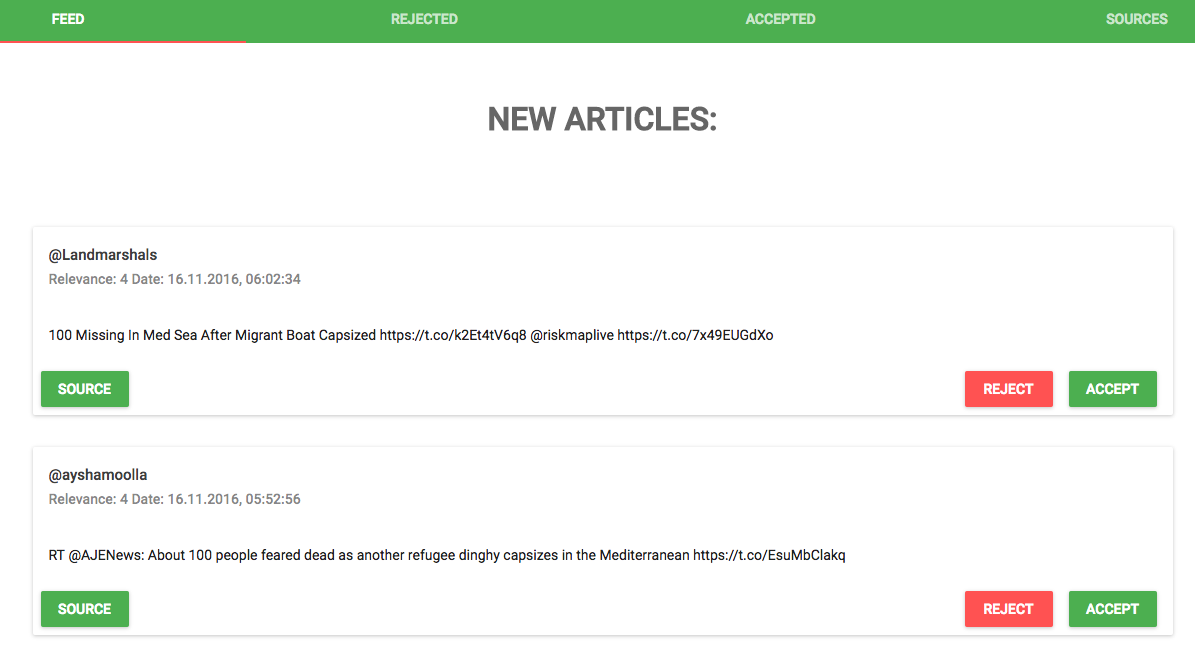
\includegraphics[scale=0.25]{UI.png}
\label{heat}
\end{figure}

\href{http://migrantnews-web.s3-website-eu-west-1.amazonaws.com/}{\beamergotobutton{Link}}

\end{frame}

%------------------------------------------------------------------------------%
%------------------------------------------------------------------------------%
\section{Text Processing}

%------------------------------------------------------------------------------%

\begin{frame}{Cleaning the strings}

\vspace{-0.5cm}

\begin{figure}[H]
\centering
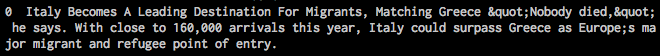
\includegraphics[scale=0.5]{Text_Processing/1.png}
\label{heat}
\end{figure}

\begin{itemize}
\item Splitting text into tokens
\end{itemize}

\vspace{-0.5cm}

\begin{figure}[H]
\centering

\includegraphics[scale=0.5]{Text_Processing/2.png}
\label{heat}
\end{figure}

\begin{itemize}
\item Removing stopwords
\end{itemize}

\vspace{-0.5cm}

\begin{figure}[H]
\centering
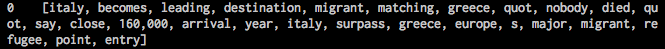
\includegraphics[scale=0.5]{Text_Processing/3.png}
\label{heat}
\end{figure}

\begin{itemize}
\item Stemming the words and converting them into lemmas
\end{itemize}

\vspace{-0.5cm}
 
\begin{figure}[H]
\centering
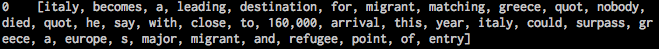
\includegraphics[scale=0.5]{Text_Processing/4.png}
\label{heat}
\end{figure}


\end{frame}
%------------------------------------------------------------------------------%

\begin{frame}{Constructing a Vectorized Representation}
\begin{itemize}
\item tf-idf: term frequency-inverse document frequency 
\item Deciding on dimensionality: bi-grams, tri-grams, etc.
	\begin{itemize}
		\item[$\to$] Which representations do really matter?
	\end{itemize}
 
\end{itemize}
\end{frame}

%------------------------------------------------------------------------------%
%------------------------------------------------------------------------------%
\section{Modelling the Data}
%------------------------------------------------------------------------------%
\begin{frame}{The Problem}
\begin{itemize}

\item Easy/accelerated classification of relevant and irrelevant news
\item Problems:
	\begin{enumerate}
		\item Redundancy: Many observations cover the same events
		\item Sensitivity: Hard classification problem
	\end{enumerate}

\item Solutions: 
	\begin{enumerate}
		\item Hierarchical clustering using DBSCAN
		\item Ensemble Methods: Random Forest
	\end{enumerate}

\end{itemize}
\end{frame}

%------------------------------------------------------------------------------%
\begin{frame}{Clustering using DBSCAN - Density-based spatial clustering of applications with noise}

\begin{itemize}
	\item Density-based clustering algorithm: core points, (density-)reachable points and outliers
	\item Core point forms cluster together with all reachable points (core or non-core).
	\item Clusters contain at least one core point; non-core points can be part of a cluster, but they form its "edge", since they cannot be used to reach more points.
	\item Applied to TF-IDF matrix and parametrized with difference tolerance 
\end{itemize}

\end{frame}

%------------------------------------------------------------------------------%
\begin{frame}{Building a First Classification Model}

\begin{itemize}
	\item Many potential classifiers available: Logistic Regression, Naive Bayes, SVM,
Decision Tree, Random Forest and Neural Networks
	\item Idea: Start with MVP (minimal viable product) to grasp the problem $\to$ Generative Model: Naive Bayes
\end{itemize}
\end{frame}

%------------------------------------------------------------------------------%
\begin{frame}{Problems in Classification}

\begin{itemize}
	\item Hyperparameter choices: 5-fold cross-validation and parameter grid search
	\item Adding non-parametric complexity: Random Forest
\end{itemize}

\end{frame}

%------------------------------------------------------------------------------%
\begin{frame}{Improving Classification}

\begin{itemize}
	\item Hyperparameter choices: 5-fold cross-validation and parameter grid search
	\item Adding non-parametric complexity: Random Forest
\end{itemize}

\end{frame}


%------------------------------------------------------------------------------%
\begin{frame}{Conclusion}

\begin{itemize}
\item Open research/work:
\begin{enumerate}
\item Better understanding of the decision boundary problem
\end{enumerate}
\item \Large{\textit{Any Questions?}}
\item \Large{\textit{Thank you for your attention!}}
\end{itemize}


\end{frame}
%------------------------------------------------------------------------------%

%\begin{frame}[allowframebreaks]{References}
 %   \begin{scriptsize}
  %   %\nocite{*}  // commented out!!!!!!!!
   %  \setbeamertemplate{bibliography item}[text]
    % \bibliographystyle{authordate1}
     %\bibliography{dynamicpanels}
    %\end{scriptsize}
    %\end{frame}

%------------------------------------------------------------------------------%

\end{document} 